\begin{frame}{Micro Model: Design}
The micro model is a discrete cellular automata model based on work from Nagel and Schrekenberg. Their model used four rules:
\begin{itemize}
\item \alert{Acceleration} If a car can accelerate up to the speed limit without hitting the car in front of it, it will.
\item \alert{Slowing down} If a car will hit the car in front of in in the next time step, it will slow down.
\item \alert{Randomization} Every car has some random probability of slowing down. (Bad driving)
\item \alert{Motion}: Each car moves forward.
\end{itemize}
\end{frame}

\begin{frame}{Micro Model: Design}
Our model modifies Nagel and Schrekenberg's original model.
\begin{itemize}
\item \alert{Acceleration} Self-driving cars can accelerate to be closer to the car in front of it.
\item \alert{Randomization} Self-driving cars have a lower probability of slowing down.
\end{itemize}
\end{frame}

\begin{frame}{Micro Model: Results}
\begin{figure}[h]
\centering
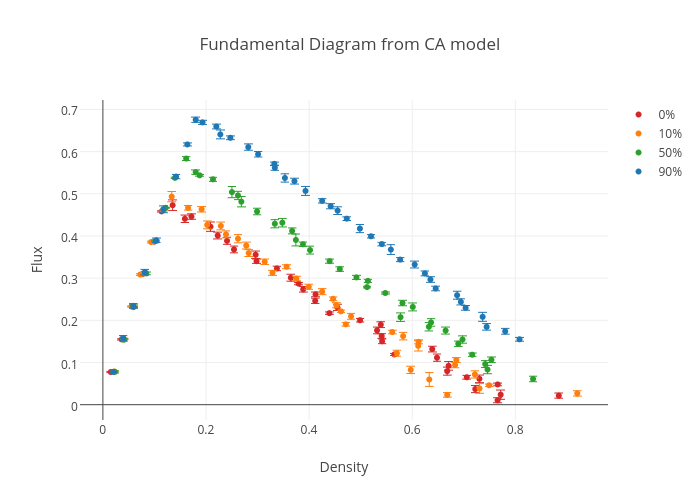
\includegraphics[width=0.9\textwidth]{img/flow-plot.png}\\
\caption{Traffic density versus traffic flux for varied proportions of autonomous vehicles in traffic predicted by the cellular automata model.}
\label{fig:flow-plot}
\end{figure}
\end{frame}

\begin{frame}{Micro Model: Results}
\begin{figure}[h]
\centering
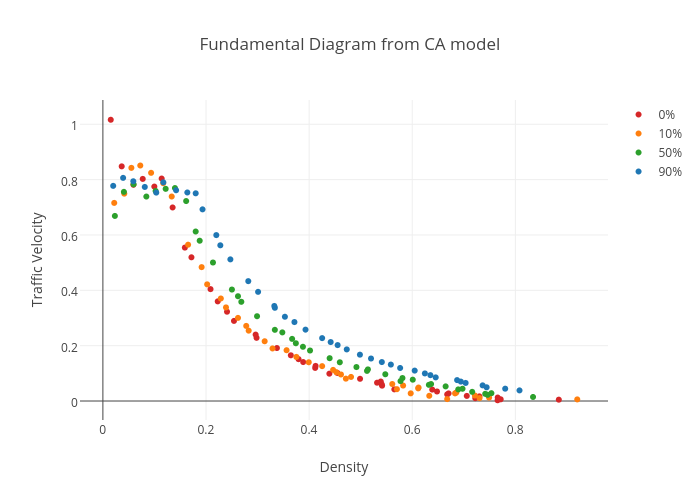
\includegraphics[width=0.9\textwidth]{img/velocity-plot.png}\\
\caption{The relationship between traffic density and traffic speed for varied proportions of autonomous vehicles in traffic predicted by the cellular automata model.}
\label{fig:vel-plot}
\end{figure}
\end{frame}